\chapter{Delay Differential Equations} \label{sec:delay-differential-equations}

\section{Piecewise Continuous Functions} \label{sec:piecewise-continuous-functions}
The following definition is motivated by capturing the character evolution arising from hybrid systems. We will see that we can consider such to be piecewise continuous.

\begin{definition}[Piecewise Continuous]
    \label{definition-piecewise-continuous}

    Let $D=[a,b]\subset\R$ be a closed interval (this includes the cases when $a=-\infty$ or $b=\infty$, or both). The mapping $x:D\rightarrow\R^n$ is called \textbf{piecewise continuous} if and only if there is a finite subdivision $\{t_i:i=0,\ldots,m\}$ of $D$ (i.e.\ $a=t_0<t_1<\ldots<t_m=b$) such that $x$ is continuous on each interval piece $[t_i,t_{i+1})$ for all $i=0,\ldots,m-1$ and the left sided limits
    \begin{equation}
        \lim_{\substack{t\nearrow t_{i+1}\\ t\in[t_i,t_{i+1})}} x(t)
    \end{equation}
    exist. Hence $x(b)$ can be an isolated point and this right interval limit $b$ is the only spot where such is allowed.

    We denote by $C^0_\text{pw}(D,\R^n)$ the set of \textbf{piecewise continuous functions} on the compact interval $D$ (this excludes the cases with $\pm\infty$), mapping to $\R^n$.

\end{definition}

% TODO: sup-norm for pw

\begin{lemma}[]
    \label{lemma-piecewise-continuous-integrable}

    A piecewise continuous function, as defined in Definition \ref{definition-piecewise-continuous} is (Riemann) integrable.
\end{lemma}

\begin{proof}
    See standard analysis literature, such as \cite{rudin1976principles} or \cite{gathmanngrundlagen}.
\end{proof}

% \begin{figure*}[h]\centering
%     \begin{subfigure}[t]{0.5\textwidth}\centering
%         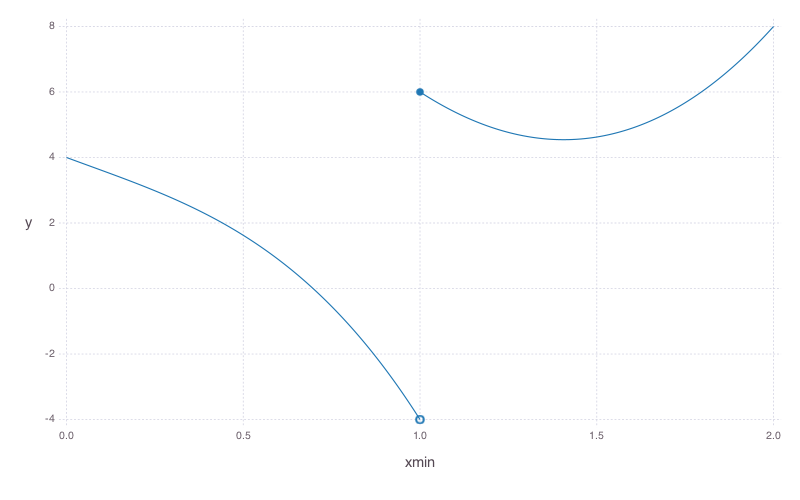
\includegraphics[width=\textwidth]{figures/allowed.png}
%         \caption{Admissible piecewise continuous function.}
%         \label{fig:allowed}
%     \end{subfigure}
%     \begin{subfigure}[t]{0.5\textwidth}\centering
%         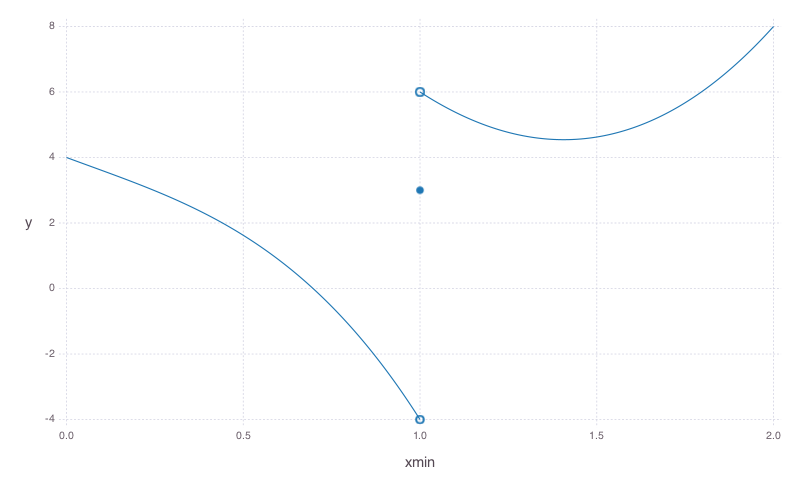
\includegraphics[width=\textwidth]{figures/not-allowed.png}
% 	    \caption{Not allowed!}
% 	    \label{fig:not-allowed}
%     \end{subfigure}
%     \caption{Examples to Definition \ref{definition-piecewise-continuous}.}
% \end{figure*}


\section{Definition DDE} \label{sec:definition-dde}

\begin{definition}[Delay Differential Equation]
    \label{definition-dde}

    Let $f:\R^n\times\R^n\rightarrow\R^n$ and $\tau > 0$.
    A functional equation of the form
    \begin{equation}
        x'(t) = f\left(x(t),x(t-\tau)\right)
    \end{equation}
    is called \textbf{Delay Differential Equation (DDE)} with \emph{constant, discrete delay}. It is \emph{autonomous}, since its right hand side $f$ is time independent.

    If the right hand side only depends on $x(t-\tau)$ and not on $x(t)$, we call the DDE \emph{pure}.

    A DDE can be equipped with an \textbf{initial condition}. It specifies the values of $x$ on $[-\tau, 0]$ on which the right hand side depends.

\end{definition}

Since we only consider autonomous DDEs, we can without loss of generality restrict to the case of initial time $t_0=0$.

The definition of a DDE can be extended to multiple constant discrete delays. For simplicity, we restrict here to a single delay.

\section{Definition of Solution} \label{sec:definition-of-solution}

\begin{definition}[Solution of DDE]
    \label{definition-solution-dde}

    A piecewise continuous function $x\in C^0_\text{pw}([-\tau,T],\R^n)$ is called \textbf{local solution} of the DDE (eq ??), if and only if there exists a $T>0$ such that $x|_{(0,T)}\in C^1((0,T),\R^n)$ with
    \begin{equation}
        x'(t) = f\left(x(t),x(t-\tau)\right)
    \end{equation}
    for all $t\in (0,T)$ and in $t=0$, it holds for the right-hand derivative \begin{equation}
        \lim_{h\searrow 0}\frac{x(h)-x(0)}{h}=f(x(0),x(-\tau))
    \end{equation}
    and obeys the initial condition:
    \begin{equation}
        x(t) = x_0(t) \quad\text{for } t\in [-\tau,0]
    \end{equation}
    on $[-\tau,0]$.

%TODO: differentiable in right rand point? need not derivative in right hand point

%TODO: Fortsetzbarkeit For example initial condition has jump, this point is limit for local solution.

    If the function $x$ is solution for all $T\in\R_{>0}$, it is called \textbf{global}.

\end{definition}

%TODO:
The notion of solution for an autonomous DDE as given above can be lifted to be a trajectory in the statespace
\begin{equation}
    \gamma_x:[0,T]\rightarrow\statespace,\\ t\mapsto\xbartaut{t}
\end{equation}

The \textbf{state} at time $t$ is a function which provides a time limited history up to the current time. This is all information needed to determine (using the DDE) to determine the solution for time $\geq t$. It is defined as $\xbartaut{t}(s)\defeq x(t+s)$ for $s\in [-\tau,0]$. In the case of $t=0$, we simplify the notation to $\xbartau \defeq \xbartaut{0}$.

This notion of solution is a \emph{dynamical systems} point of view which later turns out to be useful.

% \begin{figure}[h]\centering
%     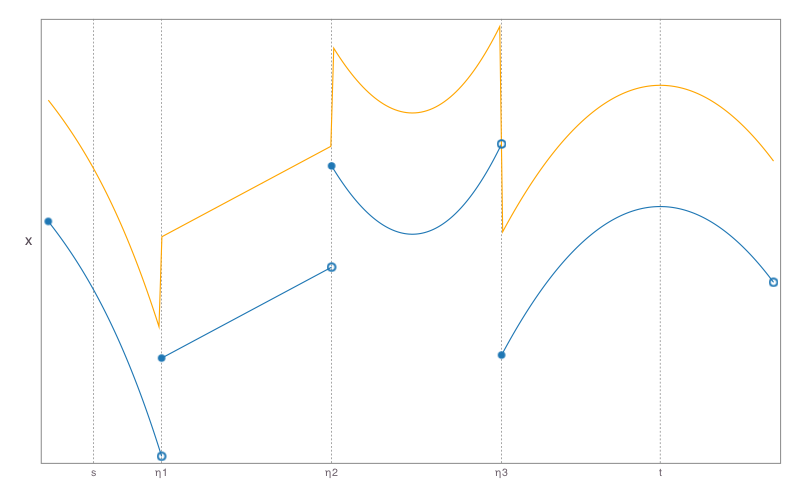
\includegraphics[width=\textwidth]{figures/multiple.png}
% 	\caption{Illustration of proof to Lemma \ref{lemma-continuity}}
% 	\label{fig:not-allowed}
% \end{figure}

% FIXME: This lemma is wrong. Show instead integrability of f(t,x_t)
\begin{lemma}
    \label{lemma-continuity}

    % Let $x:[\sigma-\tau,\sigma+T] \rightarrow \R^n$ be piecewise continuous (as in Definition \ref{definition-piecewise-continuous}) with the subdivision $\{t_0,\ldots,t_k\}$, i.e. there are $k$ subintervals.
    %
    % Then $t \mapsto x_t = x(t+\theta)$, where $\theta\in[-\tau,0]$, is a piecewise continuous mapping from $[\sigma,\sigma+T]$ into $\statespace$.
\end{lemma}

\begin{proof}
    % $x$ is piecewise continuous and hence uniformly piecewise continuous on the compact interval $I=[\sigma-\tau,\sigma+T]$.
    % i.e. uniformely continuous on each subinterval with stetiger Fortsetzung in right side.
    % \begin{equation}
    %     \forall\epsilon >0 \exists\delta_i >0 \forall t,s\in I_i: \quad \abs{t-s}<\delta_i \Rightarrow \norm{x(t)-x(s)}<\epsilon
    % \end{equation}
    % Let $\epsilon > 0$. $x|_{[t_i,t_{i+1}]}$ (with stetiger fortsetzung in right interval limit) is uniformly continuous, i.e. there is a $\delta_i > 0$ (for the given $\epsilon$), such that $\forall\,t, s \in [t_i,t_{i+1}]$ holds
    % % TODO: can use \leq ?
    % \begin{equation}
    %     \abs{t-s} < \delta_i \Rightarrow \norm{x(t)-x(s)} < \epsilon
    % \end{equation}
    %
    % Among the given $\delta_i$, choose the smallest as $\delta = \min_i \delta_i$.
    %
    % For any $i$ and $s,t\in [t_i,t_{i+1})\subset [\sigma,\sigma+T]$ with $\abs{t-s}<\delta$, it holds
    % \begin{equation}
    %     \supnorm{x_t - x_s} = \sup_{\theta\in [-\tau,0]}\norm{x(t+\theta) - x(s+\theta)} < \epsilon
    % \end{equation}
    % since $t+\theta, s+\theta \in I$
    % Hence $t \mapsto x_t$ is uniformely continuous on $[t_i,t_{i+1})$.
\end{proof}

\begin{definition}
    \label{definition-lipschitz}

    A function $f:\deff\rightarrow\R^n$ is called \textbf{locally Lipschitz continuous} in its second argument if and only if $\forall a,b\in\R,\forall M>0 \exists L>0$:
    \begin{equation}
        \norm{f(t,x,y) - f(t,\bar{x},y} \leq L\norm{x - \bar{x}}
    \end{equation}
    for all $t\in [a,b]$ and $\norm{x},\norm{\bar{x}},\norm{y}\leq M$.
\end{definition}

\begin{lemma}
    \label{lemma-bounded-f}

    Let $f:\deff\rightarrow\R^n$ be continuous and Lipschitz in its second argument.

    For any given compact interval $[a,b]$ ans $M>0$ there exists a bound $K>0$
    \begin{equation}
        \norm{f(t,x,y)}\leq K
    \end{equation}
    where $t\in[a,b]$ and $\norm{x},\norm{y}\leq M$.
\end{lemma}

\begin{proof}
    Let $L$ be the Lipschitz constant of $f$ for given $[a,b]$ and $M$. Then
    \begin{multline}
        \norm{f(t,x,y)} \leq \norm{f(t,x,y) - f(t,0,y)} + \norm{f(t,0,y)}\\
        \leq L\norm{x-0} + \norm{f(t,0,y)} \leq LM+P = K
    \end{multline}
    when $t\in[a,b]$ and $\norm{x},\norm{y}\leq M$. We used the continuity of $f$ for the existence of
    \begin{equation}
        P = \max_{s\in [a,b],y}\norm{f(s,0,y)}
    \end{equation}
\end{proof}

\begin{lemma}
    \label{lemma-integral-equation}

%TODO: solving dde equiv to solving integral equation??? (-\textgreater{} Lemma) and compare with ODE lecture notes

    Finding a solution of the DDE (??) is equivalent to solving the integral equation

    \begin{equation}
        x(t) = x_0(0) + \int_0^t g(\bar{x}_{\tau,s})ds
    \end{equation}
    and is continuous in t.
\end{lemma}

\begin{proof}
integrate from discontinuity of $\xbartaut{t}$ to discontinuity and proof stetige fortsetzbarkeit at these points
\end{proof}

\section{Method of Steps} \label{sec:method-of-steps}
for $t\in [0,\tau]$, $x$ must satisfy the following ordinary initial value problem obtained by plugging the initial function into equation (??). For suitable $f$ and $x_0$, the existence (and uniqueness) of a solution on $[0,\tau]$ is guaranteed by ODE theory (\ldots{} or Picard-Lindelöf theorems).

This procedure can then be applied repeatedly to extend the obtained solution by steps of length $\tau$.

\section{Existence and Uniqueness of Solutions} \label{existence-and-uniqueness-of-solutions}

$f$ Lipschitz with piecewise continuous initial function have existence and uniqueness ???? smoothing

\begin{theorem}
    \label{theorem-solution-existence}
    Consider the Delay Differential Equation

%TODO: do we need global existence or just local?

%TODO: this DDE is more general than in definition above

    \begin{equation}
        \begin{cases}
            x' = f(t,x(t),x(t-\tau)) & \text{for } t\geq\sigma\\
            x(t) = x_\sigma(t-\sigma)     & \text{for } t\in [\sigma-\tau,\sigma]
        \end{cases}
    \end{equation}

    with $f:\deff\rightarrow\R^n$ continuous and satisfying the (local) Lipschitz condition (\ref{definition-lipschitz}).
    % \begin{equation}
    %     \forall M>0\,\exists L>0\,\forall x,y\in C^0([-\tau,0],\R^n) : \supnorm{x},\supnorm{y}\leq M\Rightarrow\norm{f(x)-f(y)} \leq L\supnorm{x-y}
    % \end{equation}
    % where $\norm{\cdot}$ denotes the Euclidian norm on $\R^n$ and $\supnorm{\cdot}$ the supremum norm of the Banach space of continuous functions on $[-\tau,0]$.

    Then for each \textbf{initial condition} $x_\sigma\in\statespace$ and start time $\sigma$, there \textbf{exists} a \textbf{unique local solution} of the DDE on a time interval $[\sigma-\tau, \sigma+T]$. $T>0$ depends on in the initial condition, in terms of its bound and discontinuity points.
\end{theorem}
The proof is smiliar to the proof of ... given in \cite{smith2010introDDE}.
\begin{proof}
    The initial condition is bounded by $\supnorm{x_\sigma}\leq M$.
    Let $K>0$ be the bound for $f$ from Lemma \ref{lemma-bounded-f} on the set $[\sigma,\sigma+t_1] \times \{x\in R^n: \norm{x}\leq 2M\}\times \{y\in R^n: \norm{y}\leq M\}$ and $L>0$ the Lipschitz constant for that set. Choose $T=\min\{t_1-\tau ?, \frac{M}{K}\}$

    We construct a series which approximates the solution.
    Set
    \begin{equation}
        x^{(0)}(t)= \begin{cases}
            x_\sigma(0) & t\in [\sigma,\sigma+T]\\
            x_\sigma(t-\sigma) & t\in [\sigma-\tau,\sigma]
        \end{cases}
    \end{equation}
    For $m\in\N_0$ define
    \begin{equation}
        x^{(m+1)}(t)= \begin{cases}
            x_\sigma(0) + \int_\sigma^t f(s,x^{(m)}(s),x^{(m)}(s-\tau))\dx{s} & t\in [\sigma,\sigma+T]\\
            x_\sigma(t-\sigma) & t\in [\sigma-\tau,\sigma]
        \end{cases}
    \end{equation}
    It holds for all m $\forall\,t\in [\sigma-\tau,\sigma]$
    \begin{equation}
        \norm{x^{(m+1)}(t)-x^{(m)}(t)}=0
    \end{equation}
    We show by induction that
    \begin{equation}
        \norm{x^{(m)}(t)-x^{(m-1)}(t)} \leq \frac{K}{L}\frac{L^m (t-\sigma)^m}{m!}
    \end{equation}
    $\forall\,t\in [\sigma,\sigma+T]$.
    The IA holds, since obviously $\norm{x^{(0)}(t)}\leq M$
    \begin{equation}
        \norm{x^{(1)}(t)-x^{(0)}(t)} = \norm{\int_\sigma^t f(s,x^{(0)}(s),x^{(0)}(s-\tau))\dx{s}} \leq K(t-\sigma)
    \end{equation}
    Since for any $m$, it holds
    \begin{equation}
        \norm{x^{(m)}}\leq \norm{x_\sigma(0)} + \int_\sigma^t \norm{f(s,x^{(m)}(s),x^{(m)}(s-\tau))}\dx{s}
        \leq M + K(t-\sigma) \leq M+KT \leq 2M
    \end{equation}
    we can apply Lipschitz in the induction step
    \begin{align}
        \norm{x^{(m+1)}(t)-x^{(m)}(t)} &= \norm{\int_\sigma^t f(s,x^{(m)}(s),x^{(m)}(s-\tau)) - f(s,x^{(m-1)}(s),x^{(m-1)}(s-\tau))\dx{s}}\\
        & \leq K \int_\sigma^t \norm{x^{(m)}(s) - x^{(m-1)}(s)}\dx{s} \leq \frac{L^m K}{m!} \int_\sigma^t (s-\sigma)^m\dx{s}\\
        & = \frac{L^m K}{(m+1)!}(t-\sigma)^{m+1}
    \end{align}
    We use this bound and the triangle inequality in
    \begin{equation}
        \norm{x^{(t)}(t)-x^{(k)}(t)}\leq \norm{x^{(m)}(t)-x^{(m-1)}(t)} + \norm{x^{(m-1)}(t)-x^{(m-2)}(t)} +\ldots + \norm{x^{(k+1)}(t)-x^{(k)}(t)}\\
        \leq \frac{K}{L}\frac{L^m (t-\sigma)^m}{m!} + \frac{K}{L}\frac{L^{m-1} (t-\sigma)^{m-1}}{(m-1)!} +\ldots +\frac{K}{L}\frac{L^{k+1} (t-\sigma)^{k+1}}{(k+1)!}\\
        \leq \frac{K}{L}\sum_{i=k+1}^\infty \frac{(LT)^i}{i!}
    \end{equation}
    for any $k\in\N$ and $m\geq k$ and $t\in [\sigma,\sigma+T]$.
    This is the tail of the convergent exponential series and hence it converges to zero for $k\rightarrow\infty$.
    Since $x^{(m)}$ is continuous on $[\sigma,\sigma+T]$, this Cauchy sequence admits a limit $x$ in the Banach space $C^0([\sigma,\sigma+T],\R^n)$. Extend again to $[\sigma-\tau,\sigma]$ with $x_\sigma$, so $x\in C^0_\text{pw}([\sigma-\tau,\sigma],\R^n)$.


    Due to the uniform convergence of $x^(m)\rightarrow x$, we get uniform convergence of
    \begin{equation}
        f(s,x^{(m)}(s),x^{(m)}(s-\tau)) \rightarrow^{m\rightarrow\infty} f(s,x(s),x(s-\tau))
    \end{equation}
    and hence the integral and the limit process swap and by
    \begin{equation}
        x(t) = \lim_{m\rightarrow\infty} x^{(m+1)} = x_\sigma(0) + \lim_{m\rightarrow\infty}\int_\sigma^t f(s,x^{(m)}(s),x^{(m)}(s-\tau))\dx{s} = \int_\sigma^t f(s,x(s),x(s-\tau))\dx{s}
    \end{equation}
    it follows that $x$ solves the integral equation.
    This proofs the existence of a solution to the DDE. It remains to show uniqueness.

    % TODO: can one solution be on [\sigma, T_2] with T_2<T ?
    Let $x$ and $\bar{x}$ be two solutions of the DDE on $[\sigma,\sigma+T]$.
    By Lemma \ref{lemma-integral-equation} they are equivalent to solutions of the integral equations
    \begin{equation}
        x(t) = x_\sigma + \int_\sigma^t f(s,x(s,\xtau{s}))\dx{s}
    \end{equation}
    and
    \begin{equation}
        \bar{x}(t) = x_\sigma + \int_\sigma^t f(s,\bar{x}(s,x_0{\sigma-s}))\dx{s}
    \end{equation}

    For $t\in [\sigma,T]$, we set
    \begin{align*}
        \rho(t) &= \norm{x(t)-\bar{x}(t)} \leq \int_\sigma^t \norm{f()-f()}\dx{s}\\
        & \leq L \int_\sigma^t \norm{x(s)-\bar{x}(s)}\dx{s} = L \int_\sigma^t \rho(s)\dx(s)\\
        & L \int_\sigma^t \e{-\alpha s}\rho(s)\e{\alpha s}\dx{s} \leq L \sup_{s\in [\sigma,T]}(\e{-\alpha s}\rho(s))\int_\sigma^t \e{\alpha s}\dx{s}\\
        & \leq\frac{L}{\alpha}\e{\alpha s} \sup_{s\in [\sigma,T]}(\e{-\alpha s}\rho(s))
    \end{align*}
    Choosing $\alpha=2L$ and multiplying with $\e{-\alpha t}>0$ leads to
    \begin{equation}
        \rho(t)\e{-2Lt} \leq \frac{1}{2}\sup_{s\in [\sigma,T]}(\e{-\alpha s}\rho(s))
    \end{equation}
    for all $t\in [\sigma,T]$
    \begin{equation}
        0 \leq sup_{t\in [\sigma,T]}(\rho(t)\e{-2Lt}) \leq \frac{1}{2}\sup_{s\in [\sigma,T]}(\e{-\alpha s}\rho(s))
    \end{equation}
    and hence $\rho(t)=0$ for all $t\in [\sigma,T]$, which means $x(t)=\bar{x}(t)$.

    % TODO: still needed?
    just proof existence/uniqueness on each peace of continuity proof continuity at knots with Lemma of integral equ

\end{proof}

\begin{corollary}
    \label{cor:continuability-of-solution}
    If in Theorem \ref{theorem-solution-existence} $T=t_1-\tau$, can reapplay theorem with starting point $\sigma=\sigma_{old}+t_1-\tau$. Get existence of unique solution on $[\sigma-\tau,\sigma+S]$ with $S>T$.
\end{corollary}

\begin{corollary}
    \label{corollary}
    If f is polynomial in $t$, $x(t)$ and $x(t-\tau)$ then theorem holds

    polynomial -> continuously differentiable -> locally Lipschitz
% IDEA: can show? init cond bounded by M, and loc sol bounded by M, get glob sol since f glob Lip on set of bounded inputs?

%TODO: can write DDE (eq??) from definition as

\begin{equation}
    \begin{cases}
        x'=f(\xbartaut{t})\defeq g(\xbartaut{t}(0),\xbartaut{t}(-\tau)) &\text{for } t\geq 0\\
        x(t)=x_0(t) & \text{for } t\in[-\tau,0]
    \end{cases}
\end{equation}
\end{corollary}

\begin{proof}

\end{proof}

% TODO: non-autonomous -> autonomous

\section{Example}\label{example}
The basic ODE IVP
\begin{equation}
    \begin{cases}
        x'(t) = -x(t)\\
        x(0) = x_0
    \end{cases}
\end{equation}
has the solution $x(t)=x_0 e^{-t}$. However the similiar DDE
\begin{equation}
    \begin{cases}
        x'(t) = -x(t-\tau) & t\geq 0\\
        x(t) = x_0(t) & -\tau\leq t\leq 0
    \end{cases}
\end{equation}
has a much richer dynamics, but solution (as series) for $x_0\equiv 1$, can compute first solutions by method of steps. \ldots{}

\begin{figure}[h]\centering
    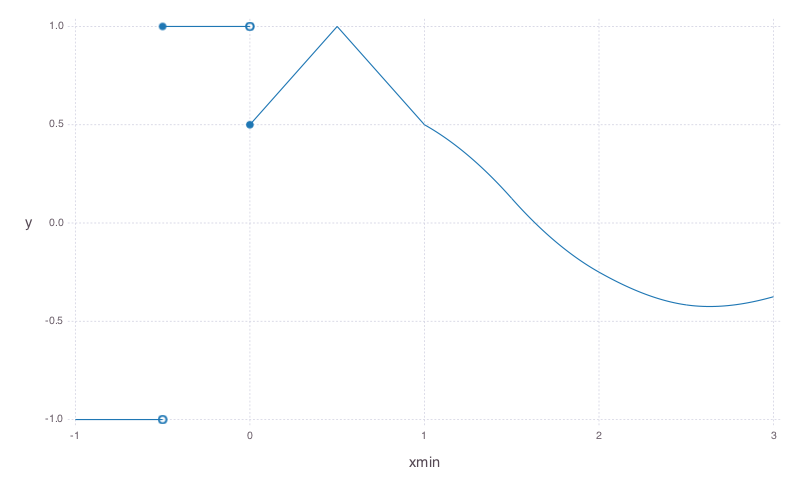
\includegraphics[width=\textwidth]{figures/piecewise-initial-function.png}
	%\caption{}
	\label{fig:not-allowed}
\end{figure}

\section{Definition}\label{definition}
